% sudo apt install texlive-lang-italian
% sudo apt install texlive-fonts-extra
% sudo apt-get install texlive-bibtex-extra biber
\documentclass[a4paper,11pt]{article}

\usepackage[utf8]{inputenc}
\usepackage[T1]{fontenc}
\usepackage[italian]{babel}
\usepackage{graphicx}

%\usepackage[backend=biber]{biblatex}
\usepackage{cv} % backbone style
\usepackage{booktabs}
\usepackage{fontawesome} % beautiful icons!!

% Change color to blue
\def\headcolor{\color[rgb]{0,0,0.5}}
% Space before section headings
\titlespacing{\section}{0pt}{2ex}{1ex}

\graphicspath{{./img/}}

\newcommand\SignatureImage[2][]{%
  \IfFileExists{#2}{%
    \includegraphics[#1]{#2}%
  }{%
    \hfill\makebox[2.0in]{\hrulefill}
  }%
}%

%\title{%
% 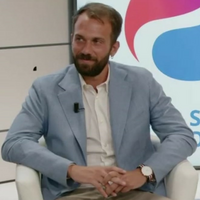
\includegraphics[width=0.1]{io.png}
%}

\name{Nico Curti}
\image{io.png}
\info{\faicon{bank} & Dept. of Experimental, Diagnostic and Specialty Medicine of Bologna University, Via Massarenti 9 Bologna\\
 \faicon{phone}     & +39 333 997 93 99\\
 \faicon{envelope}  & nico.curti2@unibo.it\\
 \faicon{github}    & \url{https://github.com/Nico-Curti}\\
 \faicon{book}      & \url{https://orcid.org/0000-0001-5802-1195}\\
}

\pagestyle{fancy}
\lhead{Curriculum vitae e scientifico-professionale}
\rhead{Nico Curti}
\rfoot{\thepage}
\cfoot{}
\renewcommand{\headrulewidth}{0.4pt}
\newcommand{\quotes}[1]{``#1''}


\begin{document}

\maketitle

\section*{\scshape{Storia accademica e scientifica}}

Nico Curti nasce a Cattolica (RN, Italia) il 28/09/1992.
Dopo aver conseguito la laurea triennale in Fisica nel 2014 presso L'Università di Bologna (BO, Italia), consegue la laurea specialistica in \emph{Fisica Applicata} (a beni culturali, ambientali, biologia e medicina) con il voto di 110/110 e lode, presentando il lavoro di tesi dal titolo \emph{Implementazione e benchmarking dell'algoritmo QDANet PRO per l'analisi di Big Data genomici}, svolto sotto la supervisione del Prof. Daniel Remondini e il Prof. Gastone Castellani dell'Università di Bologna.
Durante il lavoro di tesi, il Dr. Curti ha avuto modo di approfondire le proprie competenze algoritmiche, focalizzando il suo lavoro sull'implementazione ed ottimizzazione di codici per applicazioni su \emph{high-performance-computers}.

Successivamente, nel 2019, consegue il dottorato di ricerca in Fisica, difendendo la tesi dal titolo \quotes{Implementation and optimization of algorithms in Biological Big Data Analytics}, sotto la supervisione del Prof. Daniel Remondini, Prof. Gastone Castellani e Prof. Armando Bazzani.
Durante il lavoro di dottorato il Dr. Curti ha approfondito le sue competenze nel campo dell'\emph{intelligenza artificiale} e \emph{machine learning}, studiando i moderni modelli a rete neurale \emph{deep learning} e le più efficienti tecniche algoritmiche.
In particolare, il Dr. Curti si occupa dell'analisi di Big Data genomici mediante nuove tecniche di \emph{machine learning} e dell'applicazione di modelli a super risoluzione e segmentazione su immagini di carattere medico.
Durante il suo dottorato il Dr. Curti ha avuto l'occasione di collaborare attivamente con numerosi gruppi di ricerca di altri atenei ed è intervenuto nell'aborazione dati di numerosi progetti con enti privati.

Dal 2019 fino ad oggi è stato assegnista di ricerca presso il Dipartimento di Medicina Specialistica, Diagnostica e Sperimentale dell'Università di Bologna, sotto la supervisione del Dr. Enrico Giampieri e della Prof.ssa Emanuela Marcelli.
Durante questo periodo ha avuto modo di collaborare attivamente in numerosi progetti di carattere medico, affiancato da diversi membri delle unità ospedaliere.
In particolare, il Dr. Curti ha lavorato all'analisi di immagini istopatologiche (WSI) per la segmentazione e caratterizzazione delle componenti di melanoma, sviluppando \emph{Decision Support System}s in grado di affiancare la metodologia di valutazione tradizione durante la pratica clinica.
Inoltre ha collaborato con l'unità ospedaliera di Oftalmologia sullo sviluppo di una metodologia completamente automatizzata per la valutazione di immagini acquisite mediante lampada a fessura.


\newpage

\section*{\scshape{Titoli di Studio}}

\begin{tabular}{lp{4cm}lp{8cm}}
  2011 & Diploma                                  & Liceo Scientifico A. Volta & \\
  2014 & Laurea Triennale in Fisica               & Università di Bologna      & \emph{Integrazione di misure NMR e microscopiche per la descrizione quantitativa degli effetti di stress esterni su colture cellulari} \\
  2016 & Laurea Specialistica in Fisica Applicata & Università di Bologna      & \emph{Implementazione e benchmarking dell'algoritmo QDANet PRO per l'analisi di Big Data genomici} \\
  2019 & Dottorato in Fisica (Fisica Applicata)   & Università di Bologna      & \emph{Implementation and optimization of algorithms in Biological Big Data Analytics} \\
\end{tabular}



\vspace*{0.5cm}
\section*{\scshape{Premi, Assegni di Ricerca e riconoscimenti accademici}}

\begin{tabular}{llp{10cm}}

  2016 & Assegno di ricerca & \emph{Big Data Analytics di dati genomici e sociali high-throughput in ambiente HPC} \\
  2017 & Premio nazionale   & \emph{Premio Nazionale Giulia Vita Finzi} per la miglior tesi di laurea magistrale su attività di ricerca e sviluppo nell'ambito del calcolo dell'INFN\\
  2018 & Assegno di ricerca & \emph{Applicazione di algoritmi di machine learning nel contesto della comunicazione medico-paziente, all'interno del progetto FILOBLU} (INFN)\\
  2019 & Assegno di ricerca & \emph{Integrazione di dati clinici e multi-omici per la cura dei pazienti con patologie complesse e multisettoriali} (DIMES)\\
  2020 & Assegno di ricerca & \emph{Computer Vision ed Intelligenza artificiale per l'armonizzazione e l'analisi di imaging medico e dati multiomici} (DIMES)\\
  2021 & Assegno di ricerca & \emph{Machine learning ed Intelligenza artificiale per l'armonizzazione e l'analisi di dati multiomici del progetto HARMONY-PLUS} (DIMES)\\

\end{tabular}


\vspace*{0.5cm}
\section*{\scshape{Didattica}}

\begin{tabular}{lp{14cm}}

  2016 & Tutor presso la Scuola di Scienze dell'Università di Bologna per l'attività formativa dal titolo \emph{Analisi dati della fisica} per il corso di studi in fisica (16 ore). \\
  2020 & Professore a contratto presso la Scuola di Scienze dell'Università di Bologna per il corso di laurea in Infermieristica (abilitante alla professione sanitaria di infermiere) per il corso di \emph{Fisica Applicata}, componente del corso integrato scienze fisiologiche (24 ore). \\
  2021 & Professore a contratto presso la Scuola di Scienze dell'Università di Bologna per il corso di laurea in Infermieristica (abilitante alla professione sanitaria di infermiere) per il corso di \emph{Fisica Applicata}, componente del corso integrato scienze fisiologiche (24 ore). \\

\end{tabular}


\vspace*{0.5cm}
\section*{\scshape{Partecipazione a conferenze}}

\begin{itemize}

  \item[$\bullet$] Partecipazione alla conferenza \emph{INFN BioPhys and PlexNet}, tenutasi dal 24/09/2019 al 26/09/2019, nella quale ho presentato il lavoro dal titolo \emph{Introducing the Complex Human Interactions in MEdical Records and Atlases Network - CHIMERA}.

  \item[$\bullet$] Partecipazione alla conferenza \emph{INFN BioPhys and PlexNet}, tenutasi dal 10/09/2018 al 12/09/2018, nella quale ho presentato il lavoro dal titolo \emph{Cross-Environment comparison of a bioinformatics pipeline: perspectives for hybrid computations}.

  \item[$\bullet$] Partecipazione alla conferenza \emph{EuroPar 2018}, tenutasi dal 27/08/2018 al 31/08/2018, nella quale ho presentato il lavoro dal titolo \emph{Cross-Environment comparison of a bioinformatics pipeline: perspectives for hybrid computations}.

  \item[$\bullet$] Partecipazione alla conferenza \emph{Problems in discrete dynamics: from biochemical systems to rare events, networks, clustering and related topics - II Edition}, tenutasi dal 05/10/2017 al 07/10/2017, nella quale ho presentato il lavoro dal titolo \emph{Learning by message-passing in networks of discrete synapses the traffic congestion prediction}.

\end{itemize}


\vspace*{0.5cm}
\section*{\scshape{Corsi di formazione}}

\begin{itemize}

  \item[$\bullet$] Partecipazione alla conferenza \emph{Due seminari sul tema dell'Intelligenza Artificiale}, tenutasi il 13/06/2018, presentata dal Prof. Gianni Zanarini e dalla Prof.ssa Paola Mello.

  \item[$\bullet$] Partecipazione a \emph{Intel-Code Modernization Workshop Rome}, tenutosi dal 23/05/2017 al 24/05/2017.

  \item[$\bullet$] Partecipazione al corso di formazione presso l'INFN International School di Bertinoro dal titolo \emph{Eighth I.N.F.N. International School on architectures, tools and methodologies for developing efficient large scale scientific computing applications}, tenutosi dal 24/10/2016 al 29/10/2016.

  \item[$\bullet$] Nel periodo 30/08/2013 - 21/09/2013 ho lavorato come volontario presso la Secondary School del villaggio di Guandumehhy del distretto di Mbulu (Tanzania) come docente di matematica e fisica.

\end{itemize}


\vspace*{0.5cm}
\section*{\scshape{Tesi di laurea seguite come correlatore}}

\begin{tabular}{lllp{9cm}}

  2018 & Sofia Farina          & L-DM270  & \emph{A physical interpretation of network laplacian: role of perturbations and masses}\\
  2018 & Giovanni Marangi      & L-DM270  & \emph{Teoria dei network applicata alle strutture proteiche}\\
  2018 & Lorenzo Dall'Olio     & L-DM270  & \emph{Funzionamento di un pulsossimetro ed analisi di serie temporali pulsossimetriche}\\
  2018 & Mattia Ceccarelli     & L-DM270  & \emph{Analisi della complessità di reti neurali generate tramite algoritmi genetici}\\
  2019 & Alex Baroncini        & LM-DM270 & \emph{Sviluppo ed ottimizzazione di algoritmi per super-risoluzione ed object detection mediante deep neural network}\\
  2019 & Davide Ravaglia       & L-DM270  & \emph{Modelling social behavior of Drosophila Melanogaster under the effect of drugs}\\
  2019 & Daniele Dall'Olio     & LM-DM270 & \emph{Applicazione di un algoritmo d’apprendimento basato su sistemi fuori dall’equilibrio a dati di Genome Wide Association}\\
  2020 & Alessandro D'Agostino & LM-DM270 & \emph{Dataset generation for the training of Neural Networks oriented toward histological image segmentation}\\
  2020 & Mattia Ceccarelli     & LM-DM270 & \emph{Optimization and applications of deep learning algorithms for super-resolution in MRI}\\
  2020 & Diego Cardinali       & L-DM270  & \emph{Classification of Clausocalanus Furcatus motion utilizing the random walk theory}\\
  2021 & Davide De Paoli       & L-DM270  & \emph{Reti neurali artificiali e apprendimenti basati sulla biofisica dei neuroni}\\
  2021 & Riccardo Biondi       & LM-DM270 & \emph{Implementation of an Automated Pipeline for the Identification of Ground Glass Opacities on CT Scans of Patients Affected by COVID-19}\\
  2021 & Davide Panzeri        & LM-DM270 & \emph{AI based prediction for brightfield and stained anatomopathology}\\
  2021 & Laura Verzellesi      & LM-DM270 & \emph{Machine Learning methods for hepatocellular malignancies segmentation and MVI prediction}\\
  2021 & Giuseppe Filitto      & LM-DM270 & \emph{Implementation of an automated pipeline to predict the response to neoadjuvant chemo-radiotherapy of patients affected by colorectal cancer}\\
  2022 & Caterina Faccioli     & LM-DM270 & \emph{Spatial analysis in pathomics: a network based method applied on fluorescence microscopy}\\
  2022 & Andrea Corvina        & L-DM270  & \emph{}\\
  2022 & Stefano Bianchi       & LM-DM270 & \emph{}\\
  2022 & Giancarlo Cuticchia   & LM-DM270 & \emph{}\\
  2022 & Daniele Buschi        & LM-DM270 & \emph{}\\
  2022 & Chiara Vece           & LM-DM270 & \emph{}\\

\end{tabular}




\vspace*{0.5cm}
\section*{\scshape{Collaborazioni}}

\begin{tabular}{llp{12cm}}

  aa 2014             & Tesi Triennale  & Collaborazione con il team di ricerca MRPM guidato dalla Prof.ssa Paola Fantazzini dell'Università di Bologna, elaborando dati di imaging cellulare da me raccolti mediante microscopia ottica in contrasto di fase. Il mio contributo è stato evidenziato nella sezione Acknowledgments del paper redatto, dal titolo \emph{Water compartmentalization, cell viability and morphology changes monitored under stress by 1H-NMR relaxometry and phase contrast optical microscopy} (L. Brizi et al.), pubblicato su \emph{Journal of Physics D: Applied Physics}. \\
  aa 2016             & Tesi Magistrale & Collaborazione con il Data Center INFN-CNAF per l'implementazione ed ottimizzazione di algoritmi per l'analisi di Big Data genomici su architetture di calcolo distribuito.\\
  2016\textemdash2017 & Dottorato       & Collaborazione con Unipol Assicurazioni al fine di ottimizzare la loro rete peritale in termini di disposizione territoriale ed efficienza dei periti.\\
  2016\textemdash2017 & Dottorato       & Collaborazione con il comune di Venezia e Telecom allo studio dei flussi pedonali all'interno del comune veneziano, mediante dati geo-referenziati di telefonia mobile. \\
  2017\textemdash2018 & Dottorato       & Collaborazione con Canon e Fabbrica Digitale per lo sviluppo di tecnologie atte al rilevamento dei flussi pedonali nel comune di Venezia, che ci ha permesso di vincere il bando per il progetto \emph{Venice} in tematica \emph{smart cities}. \\
  2018\textemdash2019 & Dottorato       & Collaborazione con il centro INFN di Roma \emph{La Sapienza} allo sviluppo di algoritmi per la \emph{sentimental analysis} e il \emph{natural language processing}.\\
  2019                & Assegnista      & Collaborazione con l'Università degli Studi di Milano - Bicocca allo sviluppo di sistemi automatici per la standardizzazione della raccolta dati in microscopia a fluorescenza e seconda armonica in immagini istopatologiche.\\
  2019                & Assegnista      & Collaborazione con l'unità ospedaliera di Oftalmologia del policlinico IRCCS Sant'Orsola - Malpighi allo sviluppo di \emph{Decision Support System} per l'analisi di immagini acquisite mediante lampada a fessura.\\
  2019\textemdash2022 & Assegnista      & Collaborazione con l'unità ospedaliera di Dermatologia del policlinico IRCCS Sant'Orsola - Malpighi allo sviluppo di \emph{Decision Support System} per la segmentazione e valutazione di immagini istopatologiche.\\
  2020\textemdash2022 & Assegnista      & Collaborazione con l'unità ospedaliera di Dermatologia del policlinico IRCCS Sant'Orsola - Malpighi per la gestione ed analisi di immagini di ferite aperte e piaghe.\\
  2020\textemdash2022 & Assegnista      & Collaborazione con l'unità ospedaliera di Radiologia del policlinico IRCCS Sant'Orsola - Malpighi per la gestione ed analisi di immagini MRI, CT e PET.\\

\end{tabular}




\vspace*{0.5cm}
\section*{\scshape{Pubblicazioni}}

\begin{itemize}

  \item[$\bullet$] A. Bazzani, A. Fabbri, C. Mizzi, S. Rambaldi, F. Bertini, S. Sinigardi, \textbf{N. Curti}, R. Luzi, G. Venturi, D. Micheli, G. Muratore and A. Vannelli, \emph{Unraveling pedestrian mobility on a road network using ICTs data during great tourist events}, \emph{EPJ Data Science}, \url{10.1140/epjds/s13688-018-0168-2} (2018 Oct 22)

  \item[$\bullet$] \textbf{N. Curti} \& E. Giampieri, A. Ferraro, M. C. Vistoli, E. Ronchieri, D. Cesini, B. Martelli, D. C. Duma and G. Castellani, \emph{Cross-Environment comparison of a bioinformatics pipeline: perspectives for hybrid computations}, \emph{Euro-Par 2018: Parallel Processing Workshops}, \url{10.1007/978-3-030-10549-5_50} (2018 Dec 12)

  \item[$\bullet$] M. Malvisi \& \textbf{N. Curti}, D. Remondini, F. Palazzo, J. L. Williams, G. Pagnacco, G. Minozzi, \emph{Combinatorial Discriminant Analysis applied to RNAseq data reveals a set of 10 transcripts as signatures of infection of cattle with Mycobacterium avium subsp. paratuberculosis}, \emph{Animals}, \url{10.3390/ani10020253} (2020 Feb 5)

  \item[$\bullet$] V. Boccardi, L. Paolacci, D. Remondini, E. Giampieri, G. Poli, \textbf{N. Curti}, R. Cecchetti, A. Villa, S. Brancorsini, P. Mecocci, \emph{Cognitive decline and Alzheimer's disease in the old age: sex influence on a \quotes{cytokinome signature}}, \emph{Journal of Alzheimer's Disease}, \url{10.3233/JAD-190480} (2019 Sep 23)

  \item[$\bullet$] L. Dall'Olio, \textbf{N. Curti}, D. Remondini, Y. Safi Harb, F. W. Asselbergs, G. Castellani, H. Uh, \emph{Prediction of vascular ageing based on smartphone acquired PPG signals}, \emph{Scientific Reports}, \url{10.1038/s41598-020-76816-6} (2020 Nov 12)

  \item[$\bullet$] D. Dall'Olio \& \textbf{N. Curti}, E. Fonzi, C. Sala, D. Remondini, G. Castellani, E. Giampieri, \emph{Impact of Concurrency on the Performance of a Whole Exome Sequencing Pipeline}, \emph{BMC Bioinformatics}, \url{10.1186/s12859-020-03780-3} (2021 Feb 9)

  \item[$\bullet$] \textbf{N. Curti} \& E. Giampieri, F. Guaraldi, F. Bernabei, L. Cercenelli, G. Castellani, P. Versusa, E. Marcelli, \emph{A fully automated pipeline for a robust conjunctival hyperemia estimation}, \emph{Applied Sciences}, \url{10.3390/app11072978} (2021 Mar 26)

  \item[$\bullet$] R. Biondi \& \textbf{N. Curti}, F. Coppola, E. Giampieri, G. Vara, M. Bartoletti, A. Cattabriga, M. A. Cocozza, F. Ciccarese, C. De Benedittis, L. Cercenelli, B. Bortolani, E. Marcelli, L. Pierotti, L. Strigari, P. Viale, R. Golfieri and G. Castellani, \emph{Classification Performance for COVID patient prognosis from automatic AI segmentation – a single center study}, \emph{Applied Science}, \url{10.3390/app11125438} (2021 June 11)

  \item[$\bullet$] S. Valente, \textbf{N. Curti}, E. Giampieri, V. Randi, C. Donadei, M. Buzzi, P. Versura, \emph{Impact of blood source and component manufacturing on neurotrophin content and in vitro cell wound healing}, \emph{Blood Transfusion}, \url{10.2450/2021.0116-21} (2021 Aug 3)

  \item[$\bullet$] L. Cercenelli, M. Zoli, B. Bortolani, \textbf{N. Curti}, D. Gori, A. Rustici, D. Mazzatenta, E. Marcelli, \emph{3D virtual modeling for morphological characterization of pituitary tumors: preliminary results on its predictive role in tumor resection rate}, \emph{Applied Sciences}, \url{10.3390/app12094275} (2022 Apr 23)

  \item[$\bullet$] L. Spagnoli, M. F. Morrone, E. Giampieri, G. Paolani, M. Santoro, \textbf{N. Curti}, F. Coppola, F. Ciccarese, G. Vara, N. Brandi, R. Golfieri, P. Viale, M. Bartoletti, L. Strigari, \emph{Outcome prediction for Sars-CoV-2 patients using machine learning modelling of clinical, radiological and radiomic features derived from chest CT images}, \emph{Applied Sciences}, \url{10.3390/app12094493} (2022 Apr 28)

  \item[$\bullet$] G. Filitto, F. Coppola, \textbf{N. Curti$^\dagger$}, E. Giampieri, D. Dall’Olio, A. Merlotti, A. Cattabriga, M.A. Cocozza, M.T. Tomassoni, D. Remondini, L. Pierotti, L. Strigari, D. Cuicchi, A. Guido, K. Rihawi, A. D'Errico, F. Di Fabio, G. Poggioli, A.G. Morganti, L. Ricciardiello, R. Golfieri, G. Castellani, \emph{Automated Prediction of the Response to Neoadjuvant Chemoradiotherapy in Patients Affected by Rectal Cancer}, \emph{Cancers}, \url{10.3390/cancers14092231} (2022 Apr 29)

  \item[$\bullet$] L. Squadrani \& \textbf{N. Curti}, E. Giampieri, D. Remondini, B. Blais, G. Castellani, \emph{Effectiveness of biological inspired neural network models in learning and patterns memorization}, \emph{Entropy}, \url{10.3390/e24050682} (2022 May 12)

  \item[$\bullet$] G. Carlini \& \textbf{N. Curti}, S. Strolin, S. Fanti, D. Remondini, C. Nanni, L. Strigari, and G. Castellani, \emph{Prediction of overall survival in cervical cancer patients using PET/CT radiomic features}, \emph{Applied Science}, \url{0.3390/app12125946} (2022 June 10)

  \item[$\bullet$] E. Dika \& \textbf{N. Curti}, G. veronesi, C. Misciali, C. Ricci, G. Castellani, A. Patrizi, E. Marcelli, \emph{Advantages of manual and automatic computer-aided compared to traditional histopathological diagnosis of melanoma: a pilot study}, \emph{???}, \url{???} (2022 ???)

  \item[$\bullet$] I. Budimir, E. Giampieri, E. Saccenti, M. S. Diez, M. Tarozzi, D. Dall'Olio, A. Merlotti, \textbf{N. Curti}, D. Remondini, G. Castellani, C. Sala, \emph{Intraspecies characterization of bacteria via evolutionary modeling of protein domains}, \emph{???}, \url{???} (2022 ???)

  \item[$\bullet$] \textbf{N. Curti} \& G. Levi, E. Giampieri, G. Castellani, D. Remondini, \emph{DNetPRO: A network approach for low-dimensional signatures from high-throughput data}, \emph{???}, \url{???} (2022 ???)

  \item[$\bullet$] \textbf{N. Curti} \& G. Veronesi, E. Dika, C. Misciali, E. Marcelli, E. Giampieri, \emph{Breslow thickness: geometric interpretation, potential pitfalls, and computer automated estimation}, \emph{???}, \url{???} (2022 ???)

\end{itemize}

\vspace*{0.5cm}
\section*{\scshape{Open Access Archive}}

\begin{itemize}

  \item[$\bullet$] \textbf{N. Curti}, E. Giampieri, G. Levi, G. Castellani, D. Remondini, \emph{DNetPRO: A network approach for low-dimensional signatures from high-throughput data}, \emph{BioRxiv}, \url{10.1101/773622} (2019 Sep 19)

  \item[$\bullet$] \textbf{N. Curti} \& D. Dall'Olio, D. Remondini, G. Castellani, E. Giampieri, \emph{rFBP: Replicated Focusing Belief Propagation algorithm}, \emph{Journal of Open Source Software}, \url{10.21105/joss.02663} (2020 Oct 20)

  \item[$\bullet$] R. Biondi \& \textbf{N. Curti}, E. Giampieri, G. Castellani, \emph{COVID-19 Lung Segmentation}, \emph{Journal of Open Source Software}, \url{10.21105/joss.03447} (2021 Sep 30)

\end{itemize}


\vspace*{0.5cm}
\section*{\scshape{Conference paper}}

\begin{itemize}

  \item[$\bullet$] D. Dall'Olio, \textbf{N. Curti}, A. Bazzani, D. Remondini, G. Castellani, \emph{Classification of Genome Wide Association data by Belief Propagation Neural network}, \emph{CCS 2019}

  \item[$\bullet$] C. Mengucci \& \textbf{N. Curti}, E. Giampieri, G. Castellani, D. Remondini, \emph{Introducing the Complex Human Interactions in MEdical Records and Atlases Network - CHIMERA}, \emph{CCS 2019}

  \item[$\bullet$] C. Fiscone, \textbf{N. Curti}, M. Ceccarelli, D. N. Manners, G. Castellani, R. Lodi, D. Remondini, C. Tonon, C. Testa, \emph{Super Resolution of T$_1$w and T$_2$w MRI using deep neural networks: brain images from CamCan dataset}, \emph{GIDRM 2020}, [poster selected for oral presentation]

  \item[$\bullet$] C. Fiscone, \textbf{N. Curti}, M. Ceccarelli, D. N. Manners, G. Castellani, R. Lodi, D. Remondini, C. Tonon, C. Testa, \emph{Exploring the use of Enhanced-Deep-Super-Resolution neural network: a retrospective study on the CamCAN brain MRI Dataset}, [selected for oral communication]

\end{itemize}




\vspace*{0.5cm}
\section*{\scshape{Attività Scientifica}}

Durante il corso di laurea magistrale ho avuto modo di approfondire diverse tematiche di ricerca nel campo della biofisica e dei sistemi complessi.
Nel campo delle \emph{complex network} ho lavorato, sotto la supervisione del Prof. Daniel Remondini dell'Università di Bologna, sul tema della ricostruzione della struttura tridimensionale proteica a partire dalle mappe di contatto.
Durante questo lavoro abbiamo sviluppato un nuovo approccio per la determinazione delle coordinate 3D degli amminoacidi, ottenendo buoni risultati anche in relazione all'attuale stato dell'arte del settore.
In collaborazione con il prof. Gastone Castellani dell'Università di Bologna, ho approfondito le mie conoscenze sui modelli biologici ed evolutivi, studiando modelli di reazione-diffusione.
La mia attenzione si è focalizzata principalmente sul modello di Turing e sulla teoria di morfogenesi.
In relazione anche a questi modelli, in collaborazione con il prof. Armando Bazzani dell'Università di Bologna, ho studiato la teoria sulla ricostruzione degli attrattori del moto, sviluppando algoritmi che permettessero di sfruttare il Teorema di Takens e quindi caratterizzare l'eventuale attrattore a partire da una singola serie temporale di dati.

Durante il lavoro di tesi magistrale mi sono occupato dell'implementazione e benchmarking dell'algoritmo QDANetPRO, ideato dal team di ricerca di biofisica dell'Università di Bologna, per l'analisi di Big Data genomici.
Durante il lavoro ho potuto approfondire le mie conoscenze di machine learning, con particolare attenzione alla features extraction e features selection.
Per il benchmarking del metodo ho estratto datasets di microRNA, mRNA, Copy Number Variation e Reverse Phase Protein array dal database online \emph{The Cancer Genome Atlas}, confrontando i risultati di classificazione ottenuti con l'attuale stato dell'arte nel settore.
Una versione differente del QDANetPRO l'ho utilizzata anche per le elaborazioni dei dati di \emph{gene expression} bovino provenienti dalla collaborazione con l'\emph{Institute of Agricultural Biology and Biotechnology} di Lodi: per far fronte a diverse problematiche intrinseche nei dati ho sviluppato una versione alternativa dell'algoritmo, utilizzando metodi di teoria dei network per eseguire un'ingente riduzione della dimensionalità del problema ed estrarre una signature di geni che ha riscotrato valenza anche sul piano biologico.

Nel mio primo anno di dottorato ho potuto approfondire le mie competenze informatiche e algoritmiche.
In questo periodo ho anche avuto modo di applicare le più moderne tecniche di calcolo parallelo e distribuito, permettendo di eseguire analisi su dati anche di ingenti dimensione.
Tali codici sono stati applicati anche per l'analisi dei dati forniti da Unipol Assicurazioni, il quale richiedeva un'ottimizzazione dell'intera propria rete peritale italiana.
In parallelo a ciò ho iniziato a studiare le tecniche di apprendimento su rete neurale, proposti da R. Zecchina et al., concentrandomi sul modello di \emph{Replicated Focusing Belief Propagation}.
L'ottimizzazione del codice sviluppato da Zecchina et al. ed un suo innovativo utilizzo mi hanno permesso di analizzare i dati provenienti dall'intera rete stradale regionale emiliana e di sviluppare un metodo per la previsione degli ingorghi stradali automobilistici, in grado di fornire un'allarme fino a 30 minuti prima del verificarsi dell'ingorgo.
Tale lavoro, ancora in fase di sviluppo prima della pubblicazione, %%%%%%%%%% TODO
è stato da me presentato alla conferenza \emph{Problems in discrete dynamics: from biochemical systems to rare events, networks, clustering and related topics - II Edition}.
Insieme al flusso automobilistico ho anche iniziato ad affrontare la tematica dei flussi pedonali, riscontrando che le stesse metodologie da me precedentemente applicate per l'analisi dei geni potevano essere utilizzate anche per rilevare le strutture fondamentali del flusso pedonale cittadino.
In questo lavoro è stata sfruttata la collaborazione con il comune di Venezia e la compagnia Telecom, le quali hanno fornito i dati di tutte le celle telefoniche presenti nell'area durante giornate particolarmente problematiche come i giorni del carnevale e della festa del Redentore.
Anche quest'ultimo lavoro è ancora in fase di sottomissione. %%%%% TODO

Nel mio secondo anno di dottorato ho collaborato con il centro di calcolo CNAF per la raccolta dati e stesura dell'articolo \emph{Cross-Environment comparison of a bioinformatics pipeline: perspectives for hybrid computations}.
In questo lavoro abbiamo dimostrato l'utilizzo ed efficienza di architetture low-power per l'analisi di intere catene di genoma umano, confrontandolo con le architetture standard utilizzate nel settore della bioinformatica.
Ho collaborato inoltre con \emph{Canon} e \emph{Fabbrica Digitale} per lo sviluppo di un sistema automatico di telecamere per il monitoring dei flussi pedonali.
Studiando diversi metodi di \emph{Pattern Recognition} ho utilizzato ed ottimizzato un modello a rete neurale a convoluzione per il riconoscimento dei pedoni in sequenze video ed il loro conteggio e tracking.
In questo lavoro ho avuto modo di affrontare le problematiche relative al controllo remoto di telecamere e riguardanti l'implementazione di codice per GPUs.
Questo lavoro ha anche portato allo sviluppo di una nuova libreria per lo sviluppo di reti neurali interamente ottimizzata per il calcolo multi-threading (Byron) che ha presentato performance di calcolo spesso superiori rispetto alle implementazioni standard delle medesime architetture.

Nel mio terzo anno di dottorato ho collaborato con l'Università Sapienza di Roma all'interno di un progetto di Natural Language Processing e Sentimental Analysis per la classificazione dei messaggi tra medico e paziente.
All'interno di questo progetto ho totalmente automatizzato la comunicazione tra l'app di messaggistica e il server centrale di storage, sviluppando un servizio/demone in grado di estrarre le informazioni all'interno del database, processarle mediante algoritmi basati su reti neurali e trasmettere lo score all'app.
Questo lavoro mi ha permesso di affinare le mie competenze sulla gestione di grandi quantità di dati e di sviluppare nuovi algoritmi anche per l'analisi del linguaggio naturale.
Tali competenze sono state poi impiegate per lo sviluppo del progetto CHIMeRA (Complex Human Interaction of MEdical Records and Atlases) nel quale mediante tecniche di web-scraping ho lavorato sull'estrazione di dati da interfacce web-html andando a minare e ri-organizzare grandi database pubblici.
Questi database sono quindi stati uniti tra loro al seguito di un pesante pre-processing per l'uniformazione dei dati permettendomi di creare una struttura a network (network-of-networks) sul quale poter eseguire query e studiare legami tra gli enti a più lungo raggio rispetto al singolo database.

Nel mio primo anno da assegnista di ricerca presso il policlinico Sant'Orsola - Malpighi mi sono occupato della gestione e organizzazione di dataset medici al fine di poterli stoccare all'interno di server esterni all'area ospedaliera secondo le attuali normative sulla privacy dei dati.
In parallelo, ho collaborato con l'unità ospedaliera di Dermatologia allo sviluppo di un sistema automatico per l'analisi di \emph{Whole Slide Images} (WSI).
In questo lavoro sono state acquisite oltre 30 WSI da pazienti con diagnosi di melanoma.
Le immagini, colorate in ematossilina ed eosina (H\&E), sono state digitalizzate ed accuratamente anonimizzate dall'unità ospedaliera.
L'analisi svolta ha coinvolto la segmentazione automatica dei campioni all'interno di ciascun vetrino, la segmentazione automatica delle aree occupate dall'epidermide e dal melanoma, l'estrazione di features cliniche rilevanti per la caratterizzazione del campione a diversi livelli di scala (a partire dalla bassa risoluzione fino alla descrizione della sola componente melanocitaria, visibile solamente ai più elevanti ingradimenti), fino alla quantificazione di parametri rilevanti per la clinica istopatologica.
Questo lavoro, ancora in corso,%%%%%%% TODO
si concretizzerà a breve in pubblicazioni di carattere tecnico e clinico, in modo da coprire adeguatamente tutto le componenti del lavoro svolto.
Inoltre, ho avuto modo di collaborare con l'unità ospedaliera di Oftalmologia, ed in particolare con la prof.ssa Piera Versura, sull'analisi di immagini acquisite mediante lampada a fessura.
Questa tipologia di immagine è utilizzata quotidianamente nella pratica clinica oculistica per la stima dell'arrossamento congiuntivale del paziente.
In questo lavoro ho sviluppato un sistema interamente automatizzato per la predizione del livello di arrossamento congiuntivale, in grado di segmentare ed estrapolare la regione di interesse dalle immagini acquisite, estrarne un set di features ed infine prevederne lo score medico richiesto.
Questo lavoro si è concretizzato nella stesura dell'articolo \emph{A fully automated pipeline for a robust conjunctival hyperemia estimation}.


\vspace*{0.5cm}
\section*{\scshape{Competenze Informatiche}}

\begin{itemize}

  \item[$\bullet$] \textbf{C/C++} : ottima;

  \item[$\bullet$] \textbf{Python} : ottima;

  \item[$\bullet$] \textbf{Latex} : più che buona;

  \item[$\bullet$] \textbf{Matlab} : buona;

  \item[$\bullet$] \textbf{Bash/Powershell} : più che buona;

  \item[$\bullet$] \textbf{HTML/CSS} : buona;

  \item[$\bullet$] \textbf{JavaScript} : buona;

  \item[$\bullet$] \textbf{Java} : buona;

\end{itemize}

Inoltre ho avuto modo di utilizzare i linguaggi di programmazione \emph{Julia}, \emph{Scala} e software di rendering grafico come \emph{Blender} e \emph{MeshMixer}.


\vspace*{0.5cm}
\section*{\scshape{Competenze Linguistiche}}

\begin{itemize}

  \item[$\bullet$]\textbf{Italiano:} Madrelingua

  \item[$\bullet$]\textbf{Inglese:} livello B2

\end{itemize}


\vspace*{0.5cm}
\quad


\begin{flushright}
Bologna, \today

In fede

\vspace*{0.5cm}

\begin{figure}[h!]
  \begin{flushright}
    \SignatureImage[scale=0.5]{Firma.png}
  \end{flushright}
\end{figure}

\end{flushright}

\vspace*{\fill}
\textbf{Autorizzo al trattamento dei dati personali contenuti in questo documento ai sensi dell'articolo 13 del D. Lgs. 196/2003.}


\end{document}
